\section{Lecture 15 (April 30th)}
{\bf Chapter 4.1}\hspace{2ex}Heat Engines
\\
\begin{defi}
(Heat engine and its efficiency) A heat engine is any device that absorbs heat and converts part of that energy into work.
\begin{center}
\vspace{2ex}
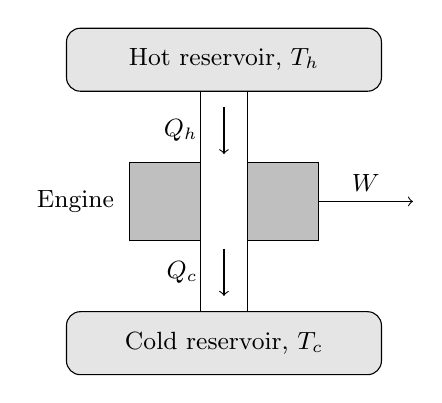
\begin{tikzpicture}[font=\small]

  % Hot reservoir
  \draw[fill=gray!20, rounded corners=5pt] (-2,1.4) rectangle (2,2.2);
  \node at (0,1.8) {Hot reservoir, $T_h$};

  % Cold reservoir
  \draw[fill=gray!20, rounded corners=5pt] (-2,-2.2) rectangle (2,-1.4);
  \node at (0,-1.8) {Cold reservoir, $T_c$};

  % Engine block
  \draw[fill=gray!50] (-1.2,0.5) rectangle (1.2,-0.5);
  \node[anchor=west] at (-2.5,0) {Engine};

  % Heat flow channel
  \draw[fill=white, draw=black] (-0.3,1.4) -- (-0.3,-1.4) -- (0.3,-1.4) -- (0.3,1.4) -- cycle;

  % Arrows for Q_h and Q_c
  \draw[->] (0,1.2) -- (0,0.6) node[midway, left=6pt] {$Q_h$};
  \draw[->] (0,-0.6) -- (0,-1.2) node[midway, left=6pt] {$Q_c$};

  % Work output arrow
  \draw[->] (1.2,0) -- (2.4,0) node[midway, above] {$W$};

\end{tikzpicture}
\vspace{2ex}
\end{center}
Take $W$, $Q_{h}$, and $Q_{c}$ to be greater than zero. The efficiency of an engine is defined as the work done over the total amount of heat provided,
\[\varepsilon =\dfrac{\mathrm{benefit}}{\mathrm{cost}}=\dfrac{W}{Q_{h}}=\dfrac{Q_{h}-Q_{c}}{Q_{h}}=1-\dfrac{Q_{c}}{Q_{h}}\]
Meanwhile, the second law of thermodynamics states that the total entropy of the engine plus its surroundings can increase but not decrease. Notice how after 1 cycle, 
\[\Delta S_{tot}=\dfrac{Q_{c}}{T_{c}}-\dfrac{Q_{h}}{T_{h}}\geq 0\]
and
\[\varepsilon =1-\dfrac{Q_{c}}{Q_{h}}\leq 1-\dfrac{T_{c}}{T_{h}}\]
\end{defi}
\vspace{2ex}
{\bf Chapter 4.2}\hspace{2ex}Refrigerator
\\
\begin{defi}
A refrigerator is a heat engine operated in reverse, where work is put in the engine and not pulled out of it. Then, heat is pushed into the Kitchen. The relevant metric is coefficient of performance (COP), 
\[\mathrm{COP}=\dfrac{\mathrm{benefit}}{\mathrm{cost}}=\dfrac{Q_{c}}{W}=\dfrac{1}{Q_{h}/Q_{c}-1}\leq \dfrac{1}{T_{h}/T_{c}-1}\]

\end{defi}
\vspace{2ex}


